%%%%%%%%%%%%%%%%%%%%%%%%%%%%%%%%%%%%%%%%%%%%%%%%%%%%%%%%%%%%%%%%%%%
%
%     McMaster University Physics & Astronomy PhD Thesis Template
%
%     filename  = "thesis.tex",
%     date      = "03/24/2015",
%     authors   = "Rory Woods",
%     copyright = "Rory Woods",
%     address   = "Physics & Astronomy,
%                  ABB,
%                  McMaster University,
%                  Hamilton, ON,
%                  CANADA",
%     telephone = "905-525-9140 ext",
%     email     = "woodsrm@mcmaster.ca",
%
%%%%%%%%%%%%%%%%%%%%%%%%%%%%%%%%%%%%%%%%%%%%%%%%%%%%%%%%%%%%%%%%%%%

\documentclass[twoside,letterpaper,phd]{macthesis}

%%%%%%%%%%%%%%%%%%%%%%%%%%%%
% Packages                 %
%%%%%%%%%%%%%%%%%%%%%%%%%%%%
\usepackage{fancyhdr}
\pagestyle{fancy}
\usepackage{deluxetable}
\usepackage{natbib} % \citet,\citep
\usepackage{aastex_hack} % Taken from: http://casa.colorado.edu/~danforth/comp/tex/thesistex.html
\usepackage{rotating}

\usepackage{amsmath}
\usepackage{amssymb}
\usepackage{amsthm}
\usepackage{exscale}
\usepackage[mathscr]{eucal}
\usepackage{bm}
\usepackage{eqlist} % Makes for a nice list of symbols.

%Rory-specific - algorithm typesetting environment
%\usepackage{algorithm2e}
\usepackage{caption}
\usepackage{subcaption}

%\usepackage[final]{graphicx}

\usepackage{epigraph}
\usepackage{lettrine}
\usepackage{keyval}

\usepackage[dvipsnames]{color}
%\usepackage{times}
%\documentstyle[fancyhdr]
%\usepackage{tabular}
%\DeclareGraphicsExtensions{.pdf, .jpg}


\usepackage{multirow}

%%%%%%%%%%%%%%%%%%%%%%%%%%%%
% Setting for fncychap     %
%%%%%%%%%%%%%%%%%%%%%%%%%%%%
% Comment out or remove the next two lines and you will get
% the standard LaTeX chapter titles. We like these A LOT
% better.
\usepackage[Lenny]{fncychap}
\ChTitleVar{\Huge\sffamily\bfseries}


%%%%%%%%%%%%%%%%%%%%%%%%%%%%%%%%%%%%
% SPECIAL SYMBOLS AND NEW COMMANDS %
%%%%%%%%%%%%%%%%%%%%%%%%%%%%%%%%%%%%
%\input{SupplementaryMaterial/UserDefinedCommands}


%%%%%%%%%%%%%%%%%%%%%%%%%%%%%%%%%%%%%%%%%
% Renewed Float Parameters              %
% (Makes floats fit better on the page) %
%%%%%%%%%%%%%%%%%%%%%%%%%%%%%%%%%%%%%%%%%
\renewcommand{\floatpagefraction}{0.85}
\renewcommand{\topfraction}      {0.85}
\renewcommand{\bottomfraction}   {0.85}
\renewcommand{\textfraction}     {0.15}



% Alter some LaTeX defaults for better treatment of figures:
% See p.105 of "TeX Unbound" for suggested values.
% See pp. 199-200 of Lamport's "LaTeX" book for detail
%   General parameters, for ALL pages:
\renewcommand{\topfraction}{0.9}	% max fraction of floats at top
\renewcommand{\bottomfraction}{0.8}	% max fraction of floats at bottom
%   Parameters for TEXT pages (not float pages):
\setcounter{topnumber}{2}
\setcounter{bottomnumber}{2}
\setcounter{totalnumber}{4}     % 2 may work better
\setcounter{dbltopnumber}{2}    % for 2-column pages
\renewcommand{\dbltopfraction}{0.9}	% fit big float above 2-col. text
\renewcommand{\textfraction}{0.07}	% allow minimal text w. figs
%   Parameters for FLOAT pages (not text pages):
\renewcommand{\floatpagefraction}{0.7}	% require fuller float pages
% N.B.: floatpagefraction MUST be less than topfraction !!
\renewcommand{\dblfloatpagefraction}{0.7}	% require fuller float pages

%=====custom commands=====%
%easy scientific notation
\providecommand{\e}[1]{\ensuremath{\times 10^{#1}}}

% ----------------------------------------------------------- %

%%%%%%%%%%%%%%%%
% FRONT-MATTER %
%%%%%%%%%%%%%%%%
% Title
\title{Seeing the Forest \emph{With} the Trees: A Novel Radiative Transfer Algorithm for Astrophysical Simulations.}
% Author and Department
\author{Rory Woods}
\dept{Physics and Astronomy}
% the degree will be conferred on this date
\degreedate{August 2015}
\copyrightyear{2015}


\documenttype{Thesis}

% This will generally be The Graduate School, though you can
% put anything in here to suit your needs.
\submittedto{The Graduate School}


%%%%%%%%%%%%%%%%%%
% Signatory Page %
%%%%%%%%%%%%%%%%%%
% You can have up to 7 committee members, i.e., one advisor
% and up to 6 readers.
%
% Begin by specifying the number of readers.
\numberofreaders{3}


\advisor[Thesis Advisor]
        {Dr. James Wadsley \& Dr. Hugh Couchman}
        {Associate Professor, McMaster University}

\readerone[Committee Member]
        {Dr. Laura Parker}
        {Associate Professor, McMaster University}

\readertwo[Committee Member]
          {Dr. Christine Wilson}
          {Professor, McMaster University}

\readerthree[External]
          {Dr. ???}
          {Professor, Somewhere Else}

% If using \include statements instead of \input statements,
% and you only want a subset of the \include statements to be
% evaluated, then declare your \includeonly here

%\includeonly{file1.tex,file2.tex,...}



%%%%%%%%%%%%%%%%%
% THE BEGINNING %
%%%%%%%%%%%%%%%%%

\begin{document}
\parindent=0.5in

%\graphicspath{{Figure/}} define figure search path

%%%%%%%%%%%%%%%%%%%%%%%%
% Preliminary Material %
%%%%%%%%%%%%%%%%%%%%%%%%
% This command is needed to properly set up the frontmatter.
\frontmatter


%%%%%%%%%%%%%%%%%%%%%%%%%%%%%%%%%%%%%%%%%%%%%%%%%%%%%%%%%%%%%%
% IMPORTANT
%
% The following commands allow you to include all the
% frontmatter in your thesis. If you don't need one or more of
% these items, you can comment it out. Most of these items are
% actually required by the Grad School -- see the Thesis Guide
% for details regarding what is and what is not required for
% your particular degree.
%%%%%%%%%%%%%%%%%%%%%%%%%%%%%%%%%%%%%%%%%%%%%%%%%%%%%%%%%%%%%%
% !!! DO NOT CHANGE THE SEQUENCE OF THESE ITEMS !!!
%%%%%%%%%%%%%%%%%%%%%%%%%%%%%%%%%%%%%%%%%%%%%%%%%%%%%%%%%%%%%%

% Generates the signature page. This is not bound with your
% thesis.
%\macsigpage


% Generates the committee page -- this is bound with your
% thesis. If this is an baccalaureate honors thesis, then
% comment out this line.
%\maccommitteepage


% Generates the title page based on info you have provided
% above.
\mactitlepage


% Generate the descriptive note page: Short-title page
\descriptivenote{supplementary/DescriptiveNote}


% Generates the abstract. The argument should point to the
% file containing your abstract.
\thesisabstract{supplementary/Abstract}

% Generates the Epigraph/Dedication. The first argument should
% point to the file containing your Epigraph/Dedication and
% the second argument should be the title of this page.
\thesisdedication{supplementary/Dedication}{}

%\thesiscoauthorship{supplementary/Coauthorship}

\thesisacknowledgments{supplementary/Acknowledgments}

\thesisepigraph{supplementary/Epigraph}


% Generates the Table of Contents
\thesistableofcontents



% Generates the List of Figures
\thesislistoffigures



% Generates the List of Tables
\thesislistoftables



% Generates the List of Symbols. The argument should point to
% the file containing your List of Symbols.
%\thesislistofsymbols{supplementary/ListOfSymbols}

% Generates the Acknowledgments. The argument should point to
% the file containing your Acknowledgments.
%\thesisacknowledgments{supplementary/Acknowledgments}





%%%%%%%%%%%%%%%%%%%%%%%%%%%%%%%%%%%%%%%%%%%%%%%%%%%%%%
% This command is needed to get the main part of the %
% document going.                                    %
%%%%%%%%%%%%%%%%%%%%%%%%%%%%%%%%%%%%%%%%%%%%%%%%%%%%%%

%\thesisepigraph{supplementary/Epigraph}


\thesismainmatter

%%%%%%%%%%%%%%%%%%%%%%%%%%%%%%%%%%%%%%%%%%%%%%%%%%
% This is an AMS-LaTeX command to allow breaking %
% of displayed equations across pages. Note the  %
% closing the "}" just before the bibliography.  %
%%%%%%%%%%%%%%%%%%%%%%%%%%%%%%%%%%%%%%%%%%%%%%%%%%
\allowdisplaybreaks{
%
%%%%%%%%%%%%%%%%%%%%%%
% THE ACTUAL CONTENT %
%%%%%%%%%%%%%%%%%%%%%%
% Chapters
%\begin{singlespace}
\begin{doublespace}
\pagestyle{fancy}
\headheight 20pt
\lhead{Ph.D. Thesis --- R. Woods}
\rhead{McMaster - Physics \& Astronomy}
\chead{}
\lfoot{}
\cfoot{\thepage}
\rfoot{}
\renewcommand{\headrulewidth}{0.1pt}
\renewcommand{\footrulewidth}{0.1pt}

\chapter{Introduction}
\label{chap:intro} 
\thispagestyle{fancy} 

It doesn't take much to convince a physicist of the importance of photons - astrophysical objects speak in photons. As astronomers, we receive all of our information in the universe through photons. In order to understand the objects we observe, we must understand photons; how are they created? How are they removed? What processes can alter a photon? To answer these questions, let's explore some of the many objects and photon energies present in astrophysics.

\section{Astrophysics and Radiation}
\label{sec:astroandrad}



\begin{itemize}
\item FUV - 6.2-10.16 ev -
\item Ly$\alpha$ - 10.16-10.25 - 
\item EUV - 12.4 - 124 ev - 
\item Soft X-rays - 124 ev - 5 kev - 
\item hard X-rays - 5-10 kev
\item IR - 1.24mev - 1.7 ev - 
\item Cosmic Rays - ...
\end{itemize}




%
%\begin{itemize}
%\item Introduce stellar systems -  radiation can provide pressure support, can cause ionization, dissociation, can heat the gas. Because gas properties tied to star formation rate, and stars are one of the primary targets of observation, it's important to know what's going on.
%\item Introduce cosmology (how in depth here?). Cosmology depends on knowing photon history and what cosmological factors affect photons. Introduce cosmic reionization, Universe expansion, SZ?, lensing?, CMB?
%\item Need to ability to track photoionization, photoheating across huge amounts of sources and their environments. Astrophysical radiation has both short and large scale effects that can't be ignored.
%\end{itemize}

%[abelnormanmadau has good cosmo-intro w/ references.]


%Introduction to the basics of cosmology
%·         properties in the context of computational radiative transfer
%
%·         important evends like re-ionization of the universe
%
%·         ionization fronts and large numbers of sources
%
%·         with a focus on the physics side of things
%
% 
%Astro relies on photons - language of the universe
%·         only way the universe can be observe
%
%·         needs to be understood to get an idea of how things are interacting
%
% 
%Look at cosmology and stellar systems where these things are really important. 
%·         In order to understand why the algorithm needs to function the way it does, need to understand cosmology to have relevant applications
%
%·         Need to develop a what to represent approximations to deal with the large length scales and large number of sources.


%First part - what is this document? What will be in it? What is the main thing I will be telling you about? [Move this after intro to astro stuff? I think so...].



\section{Overview}

Chapter \ref{chap:radtransfer} will go over the background of radiative transfer and the currently available codes that solve the radiative transfer problem. It will also motivate the need for a new code in a particular niche. Chapter \ref{chap:method} will introduce the new radiative transfer method that we have developed. Chapter \ref{chap:codetests} will demonstrate the strengths and weaknesses of the new algorithm through a variety of numerical and phyical tests. Chapter \ref{chap:galaxyformation} will show the results of using the algorithm on an isolated galaxy in the FUV band, and will also focus on future projects that the algorithm will be used for. Finally, chapter \ref{chap:conclusions} contains the conclusions of this thesis.

\pagestyle{fancy}
\headheight 20pt
\lhead{Ph.D. Thesis --- R. Woods}
\rhead{McMaster - Physics \& Astronomy}
\chead{}
\lfoot{}
\cfoot{\thepage}
\rfoot{}
\renewcommand{\headrulewidth}{0.1pt}
\renewcommand{\footrulewidth}{0.1pt}

\chapter{Radiative Transfer}
\label{chap:radtransfer}

\thispagestyle{fancy}

This chapter will contain an overview of current radiative transfer methods and where we stand.

\section{The Radiative Transfer Problem}
\label{sec:rtformulation}

When considering the transfer of photons, we must consider the scale we are dealing with. At the individual photon level, propagation is described by classical electrodynamics. Once we get to larger scales, however, it is more useful to treat radiation in ``packets'' or as an energy flux.

Consider an infinitesimal patch of area, dA, normal to a direction $\hat{n}$. We consider an infinitesimal solid angle, $d\Omega$, and consider all rays passing through the area and within the solid angle (see figure \ref{fig:intensity}).

\begin{figure}
\label{fig:intensity}
\includegraphics[width=\textwidth]{graphics/placeholder.eps}
\caption{The geometry for all rays at a point p through area dA within solid angle $d\Omega$.}
\end{figure}

The energy through this area patch, within the solid angle, in time dt, and within the frequency range $d\nu$ is

\begin{equation}
\label{eq:intensity}
dE = I_{\nu}dA dt d\Omega d\nu,
\end{equation}

where $I_{\nu}$ is \emph{specific intensity} (specific because it is within a frequency range; dropping the frequency dependence makes this intensity). Specific intensity has units of energy per unit area per unit time per unit solid angle per unit frequency. It is useful to consider radiation in terms of intensity because it enables a macroscopic description of radiation that includes microscopic effects like scattering and absorption.

We can recover familiar values such as flux (or pressure or density) by taking moments of the intensity,

\begin{equation}
\label{eq:flux}
F_{\nu} = \int I_{\nu}\cos{\theta}d\Omega,
\end{equation}

where $F_{\nu}$ is the specific flux (flux at a particular wavelength).

Let us now consider the passage of these rays through some matter. If we consider a ray, then energy may be added or removed from this ray due to absorption (removing photons), emission from the matter (adding photons), or scattering (scattering into or out of the ray). We first consider emission.

We define the specific (monochromatic) emission emission coefficient, j, as the energy emitted per unit time, per unit solid angle, per unit volume, and per unit frequency,

\begin{equation}
\label{eq:emissioncoef}
dE = j_{\nu} dV dt d\Omega d\nu.
\end{equation}

If we trace along a ray with cross section dA some distance ds, it will cover a volume of $dV = dA ds$. Since equation \ref{eq:emissioncoef} and equation \ref{eq:intensity} only differ by a factor of distance (dA compared to dV), we can find the change intensity along the beam due to emission as

\begin{equation}
\label{eq:emissionintensity}
dI = j_{\nu} ds.
\end{equation}

Equation \ref{eq:emissionintensity} describes the amount of intensity added to a ray along some path ds due to spontaneous emission. If emission were the only process to worry about, finding intensity would be a simple matter of integrating the equation. [However, we must consider other physical processes for a more complete description.]

We next consider absorption. Consider again a ray traveling along a path ds. The amount of intensity lost due to absorption can be defined as

\begin{equation}
\label{eq:absorption}
dI = -\alpha I ds,
\end{equation}

where $\alpha$ is called the absorption coefficient and has units of distance$^{-1}$. It can be shown \citep{rybickiLightman86} that $\alpha$ is a function of more commonly known variables,

\begin{equation}
\label{eq:absorptioncoeff}
\alpha = -n \sigma I ds = -\rho \kappa I ds
\end{equation}

where n is the number density of particles, $\sigma$ is the cross section (in units of distance squared) of each absorbing particle, $\rho$ is the mass density, and $\kappa$ is the opacity (in units of distance squared per unit mass). Notice that the only difference between $n \sigma$ and $\rho \kappa$ is the average mass of the absorbing particles. Note that our algorithm has chosen to use $\rho$ and $\kappa$.

Finally, we consider scattering. Scattering is a process that both subtracts and adds to the intensity. We can define a specific emission coefficient for scattering by equating the power per unit volume per frequency emitted to the power received,

\begin{equation}
\label{eq:scatteringcoefficient}
j_{s,\nu} = \sigma_{\nu} J_{\nu},
\end{equation}

where $\sigma_{\nu}$ is the specific scattering coefficient, and $J_{\nu}$ is the specific mean intensity, defined as

\begin{equation}
\label{eq:meanintensity}
J_{\nu} = \frac{1}{4\pi}\int I_{\nu} d\Omega.
\end{equation}

Before combining all of the processes affecting radiative transfer, it is useful to introduce a variable called the specific \emph{Source Function},

\begin{align}
\label{eq:sourcefunction}
S_{a,\nu} &\equiv \frac{j_{\nu}}{\alpha_{\nu}},\\
S_{s,\nu} &\equiv \frac{j_{\nu}}{\alpha_{\nu}}.
\end{align}

The source function is the ratio of emission to absorption and describes the intensity that an object will tend to. In the case of pure absorption, emission is 0 and so the source function is 0, since the intensity would tend to 0. In the case of pure emission, the source function is infinite and intensity tends to infinity since nothing is removing photons.

We now have the base equations to put together a description of radiative transfer that includes the processes of spontaneous emission, absorption, and scattering. Combining equations \ref{eq:emissionintensity}, \ref{eq:absorption}, \ref{eq:scatteringcoefficient}, \ref{eq:meanintensity}, and \ref{eq:sourcefunction}, we can write

\begin{align}
\label{eq:combinedtransfer}
\frac{dI_{\nu}}{ds} &= (-\alpha_{\nu}I_{\nu} + j_{\nu}) - (\sigma_{\nu}I_{\nu} + j_{s,\nu}) \nonumber\\
 &= -\alpha_{\nu}(I_{\nu} - S_{a,\nu}) - \sigma_{\nu}(I_{\nu} - S_{s,\nu}) \nonumber\\
 &= -(\alpha_{\nu} + \sigma_{\nu})(I_{\nu}-S_{\nu}),
\end{align}

where the combined source function $S_{\nu}$ is defined as

\begin{equation}
\label{eq:combinedsourcefunction}
S_{\nu} \equiv \frac{\alpha_{\nu}S_{a,\nu} + \sigma_{\nu}S_{s,\nu}}{\alpha_{\nu} + \sigma_{\nu}}.
\end{equation}

According to equation \ref{eq:scatteringcoefficient}, the source function for scattering is actually mean intensity (equation \ref{eq:meanintensity}), meaning that the above equation is actually an integro-differential equation - it is a function of $I_{\nu}$, $\frac{dI_{\nu}}{ds}$, and $\int I_{\nu} d\Omega$. Thus, any equation involving scattering is significantly more difficult to solve. Numerical solutions to integro-differential equations are usually specialized and complex [cite someone].

For this reason, scattering is often omitted from radiative transfer solver due to very large added computational cost. In this thesis, our solutions do not explicitly account for scattering, though it is possible scattering-like behavior (due to properties of the RT algorithm and the properties of SPH) may result in some solutions [remove this line I think].

If scattering is omitted, equation \ref{eq:combinedtransfer} is simplified to a nicer form. We combine equations \ref{eq:emissionintensity}, \ref{eq:absorption}, and \ref{eq:sourcefunction} to obtain

\begin{equation}
\label{eq:transferequation_s}
\frac{dI_{\nu}}{ds} = -\alpha_{\nu}I_{\nu} + j_{\nu}.
\end{equation}

It is now useful to introduce optical depth $\tau_{\nu}$,

\begin{equation}
\label{eq:opticaldepth}
\tau(s) = \int_{s_0}^{s} \alpha_{\nu}(s')ds' = \int_{s_0}^{s} \reveryho(s') \kappa_{\nu}(s') ds'.
\end{equation}

Optical depth is a unitless value that describes the mean free path of a photon between interactions. The distance needed in the integral to give $\tau_{\nu} = 1$ should correspond to one mean free path given the absorption coefficient $\alpha_{\nu}$. It is useful to rewrite equation \ref{eq:transferequation_s} in terms of $\tau_{\nu}$ and $S_{\nu}$ by simply dividing by $\alpha_{\nu}$

\begin{equation}
\label{eq:transferequation_t}
\frac{dI_{\nu}}{d\tau_{\nu}} = -I_{\nu} + S_{\nu}.
\end{equation}

Equation \ref{eq:transferequation_t} is the transfer equation for radiation as it is most commonly seen. A solution can be obtained by using an integrating factor of $e^{\tau_{\nu}}$, which gives the formal solution to the transfer equation

\begin{equation}
\label{eq:transferequationsolution}
I_{\nu}(\tau_{\nu}) = I_{\tau}(0)e^{-\tau_{\nu}} + \int_0^{\tau_{\nu}} e^{-(\tau_\nu - \tau'_{\nu})} S_{\nu}(\tau'_{\nu})d\tau'_{\nu}.
\end{equation}

Solving the above equation at a point in a simulation would give you a radiation field that accounted for emission and absorption at all other points in the simulation. This would then be repeated at all points for which a radiation field should be known.

It should now be clear why radiative transfer is a difficult problem; analytically, it involves integrals over source functions that are not necessarily known at all points in space, with both density and opacity varying as a function of position as well. Numerically, we are trying to solve a function of seven variables - three position, two angular, time, and frequency - $I = I(x,y,z,\theta,\phi,t,\nu)$.

[Add further simplifications to the equation here? Just talk about the absorption solution? Mention that integrating over all emission typically amounts to summing over all sources.]

%\begin{equation}
%\label{eq:rademission}
%I(s) = I(s_0) + \int_{s_0}^{s} j(s') ds'
%\end{equation}
%
%\begin{equation}
%\label{eq:radabsorption}
%I(s) = I(s_0)\exp{\left[-\int_{s_0}^{s} \alpha(s') ds'\right]} = I(s_0)\exp{\left[ -\tau (s) \right]}
%\end{equation}

\section{Current Methods}
\label{sec:currentmethods}

The equations presented in section \ref{sec:rtformulation} are very difficult to solve if approximations are not made. Seven dimensions means that even if each dimension only has a resolution of 100 elements, we must keep track of $10^14$ elements, or roughly one petabyte of data if each element is 10 bytes. In many cases, 100 elements is not nearly fine enough to resolve important features in a dimension, especially in frequency where many sharp features are present. The problem is already numerically impractical from a memory perspective.

As well, the transfer equation is an integro-differential equation, meaning that common numerical solvers are not useful. Solvers for this type of equation are generally complex and specific purpose, so the actual numerical method side is also difficult.

In order to overcome the above, different approximations to the equation are adopted. Different approximations give rise to different advantages and disadvantages in accuracy and speed and typically apply best to particular regimes.

Current popular strategies include monte-carlo, ray tracing, grid-based solvers, and moment methods. The following sections will give a brief description of each method as well as common properties of the methods.

\subsection{Monte-Carlo Solvers}
\label{montecarlo}

Monte-Carlo methods are perhaps the most obvious way to solve the radiative transfer problem. The most basic solution follows a photon from emission, through any scattering, until it leaves the simulation. At any point during the path, random numbers are used to determine whether the photon will be scattered, what direction it will be scattered, whether it will be absorbed and re-emitted, and what wavelength the re-emitted photon(s) will be.

In practice, following individual photons is not practical. Instead, following ``photon packets'' is more useful. Packets are typically defined as a group of photons [cite codes that do this] or as having a specified energy (in which case, the number of photons can be determined by using $E = h\nu$). The latter choice has the benefit that when re-emission occurs after an absorption at a lower wavelength, there are not now more photons to keep track of. The ray retains the same energy and more photons are implied since $\nu$ changes \citep{ercolanoEt03,abbottLucy85}.

% calculate random distance based on relation between random number and normalized optical depth - harries and howarth 97
% or, ask probability at each new cell that it is absorbed - Lucy 1999.
% first method more expensive - ercolano et al 2003

%estimator is needed - MC provides means to relate quantities we observe to physical quantities we want to determine. Need measure of mean intensity. See eq 9 in ercolano 03 for estimator from Och et al 98. Also create new estimator.

%Emission happens as sampled from local gas spectrum.

%process is iterative. When photons have all been sent, can iterate with estimator from above and local ionization state to converge on values.

%can finally use results to make observations if desired (usually primary use of this method).





%In monte-carlo methods, a photon is carefully tracked through a domain, following scattering, absorption, and re-emission. See [from steinacker 09] \citet{wolf03,woodEt2004,ercolanoEt2005,jonsson06,pinteEt06}. [ADD method basics]

%\begin{itemize}
%\item Advantages - can treat complicated spatial distributions, arbitrary scattering functions, and polarization.
%\item Disadvantages - Very high or low optical depths hard (why?), re-emission in all directions over many events hard (why?), no global error control
%\end{itemize}


\subsection{Ray Tracing}
\label{sec:raytracing}

Ray tracing has the ability to treat arbitrary density distributions, and can use general solvers for ODEs. Fairly accurate and fairly expensive.

\begin{itemize}
\item Often combined with monte-carlo methods
\item Provides quite accurate results.
\item Provides global error control.
\item Can cause step-size limitations in order to consistently transfer photons.
\item Becomes impractical at high optical depth and can require complicated solvers.
\end{itemize}


\subsection{Grid-Based Methods}
\label{sec:gridmethods}

Can use simple solvers (finite differencing or short characteristics) and gives good error control.

\begin{itemize}
\item Grid must be adaptable to be practical, though good refinement criteria is unclear
\item Interpolation between grids can be costly and give interpolation errors.
\item Numerical diffusion typically not taken into account.
\end{itemize}


\subsection{Moment Methods}
\label{sec:momentmethods}

e.g. FLD or M1 moment codes (skinner + ostriker, others). Fairly accurate, faster than ray tracing, in specific regimes.

\begin{itemize}
\item Well suited for optically thick regime (can do free streaming)
\item Struggles with peaked radiation in optical depths of order 1.
\end{itemize}

\subsection{Summary of Methods}
\label{sec:summaryofmethods}


%The current set of computational methods can be classified as follows:
%
%\begin{itemize}
%\item Very accurate, expensive methods - monte carlo, ray tracing
%\item Methods accurate in specific scenarios, e.g. FLD for optically thick, ``str\"omgren method'' from Dale
%\item \emph{Very} rough approximations, e.g. method that only looks at absorption near sink and source.
%\end{itemize}
%
%As will be seen, there is currently an opening in the market for something in the middle - Decent accuracy at a low cost.


\pagestyle{fancy}
\headheight 20pt
\lhead{Ph.D. Thesis --- R. Woods}
\rhead{McMaster - Physics \& Astronomy}
\chead{}
\lfoot{}
\cfoot{\thepage}
\rfoot{}
\renewcommand{\headrulewidth}{0.1pt}
\renewcommand{\footrulewidth}{0.1pt}

\chapter{The Numerical Method}
\label{chap:method}
\thispagestyle{fancy}



\section{Tree Data Structures}

\subsection{kd-Tree}

\section{Building a Radiation Tree}

\subsection{Criteria for Opening Cells}

\subsection{Accumulating Cell Properties}

\section{The Simple Case - No Absorption}

\subsection{Exchanging Radiation}

\section{Adding Absorption}

\subsection{Making Use of the Tree}

\section{Refinement}

\subsection{Criteria to Refine}

\section{Resolving the Sending and Receiving Cells}

\pagestyle{fancy}
\headheight 20pt
\lhead{Ph.D. Thesis --- R. Woods}
\rhead{McMaster - Physics \& Astronomy}
\chead{}
\lfoot{}
\cfoot{\thepage}
\rfoot{}
\renewcommand{\headrulewidth}{0.1pt}
\renewcommand{\footrulewidth}{0.1pt}


\chapter{Code Tests}
\label{chap:codetests}
\thispagestyle{fancy}

In this chapter, I present tests to demonstrate the strengths and limitations of the above algorithm.

\section{Glass}
\label{sec:glass}

A glass of particles is a simple way to demonstrate the most basic functionality of the algorithm. Each particle effectively acts to sample the radiation field at a particular point and has an easily calculated exact solution to compare to.

\subsection{Optically Thin}
\label{sec:thinglass}

{TAKE THIS SECTION OUT? TOO SIMPLE?}

In the optically thin case, we simply want to ensure that we obtain a $1/r^2$ dropoff with flux. There should be no errors present in this test case because in the case of a single source, no averaging is needed and both exact luminosity and position of the source is used for every sink.

\begin{equation}
\label{eq:flux}
F = \frac{L}{4\pi r^2}
\end{equation}

\subsection{Optically Thick}
\label{sec:thickglass}

{TAKE THIS SECTION OUT? TOO SIMPLE?}

Like section \ref{sec:thinglass}, this section aims to demonstrate the base ability of the code. In this case, the glass of particles has a roughly homogeneous density and thus the flux is still easily calculated for comparison.

\begin{itemize}
\item The equation for flux in this case is still fairly simple. If we refer to equation \ref{eq:radabsorption}, we can see the theoretical flux is simply equation \ref{eq:flux} multiplied by the exponential of optical depth. See equation \ref{eq:thickflux}.
\item This assumes a homogeneous density field. The glass does not have an exactly homogeneous field, but has little variance from the average.
\item Figure \ref{fig:thickglasserrors} shows the error distribution of the particles.
\item Note that in the case that the density field is exact, the errors reduce down to machine precision. This emphasizes the importance of accurately modeling the density distribution.
\end{itemize}

\begin{equation}
\label{eq:thickflux}
F = \frac{L}{4\pi r^2} \exp{-\tau}
\end{equation}

\begin{figure}
\includegraphics[width=\textwidth]{graphics/placeholder.eps}
\caption[Error distribution for a single source in a uniform field.]{The distribution of flux errors among particles.}
\label{fig:thickglasserrors}
\end{figure}

\section{Multi-Source Glass}
\label{sec:multiglass}

We now show the effect of including many sources. The code is now performing at its most ``stressed;'' having a large number of randomly distributed sources means the code will run at its slowest and will include a large amount of averaging (not quite right).

\begin{itemize}
\item We first present the optically thin case. In this case, the glass has had half of its gas particles replaced with sources so that there are an equal number of each.
\item The error distribution present in this
\end{itemize}

\section{Effects of Averaging the Source}
\label{sec:averagingsource}

We now look closely at what effects averaging sources can have on results.

\subsection{Two star}
\label{sec:twostar}



\subsection{Isothermal Sphere with a Cluster}
\label{sec:cluster}



\section{The Str\"omgren Sphere}
\label{sec:stromgren}



\subsection{The Isothermal Case}
\label{sec:isostromgren}



\subsection{The Thermal Case}
\label{sec:thermalstromgren}



\section{The Gas Wall}
\label{sec:gaswall}



\subsection{Only Radiation}
\label{sec:gaswallradonly}



\subsection{With Hydrodynamics - the Champagne Flow}
\label{sec:champagne}



\section{Shadowing}
\label{sec:shadowing}



\section{Galaxy Disk}
\label{sec:galaxydisk}



\section{Timings and Scaling}
\label{sec:timing}




\pagestyle{fancy}
\headheight 20pt
\lhead{Ph.D. Thesis --- R. Woods }
\rhead{McMaster - Physics \& Astronomy}
\chead{}
\lfoot{}
\cfoot{\thepage}
\rfoot{}
\renewcommand{\headrulewidth}{0.1pt}
\renewcommand{\footrulewidth}{0.1pt}

\chapter{Applications to Galaxy Formation and Future Projects}
\label{chap:galaxyformation}
\thispagestyle{fancy}

We now use the algorithm described in chapter \ref{chap:method} and tested in chapter \ref{chap:codetests} to carry out simulations of an isolated galaxy. We have chosen to start with an isolated galaxy in order to probe the FUV field present in a [Milky Way-like... z=1?] disk in order to check if it is an important SF regulation mechanism.

FUV is an interesting band to start with for a few reasons. While FUV does not ionize gas, it is the primary driver of photoelectric heating \citep{tielens05}, which is the dominant heating mechanism for the ISM and the warm neutral medium. Despite this, very few astrophysical simulations actually include photoelectric heating due to its dependence on a radiation field.

As well, FUV is typically able to penetrate further into the ISM. At common densities in the ISM, an optical depth of 1 is typically only achieved after roughly one kpc. Current simulations, especially of isolated galaxies, can resolve distances much smaller than this, so looking at effects due to FUV is very feasible. On the other hand, bands such as EUV are usually absorbed within a few pc, a resolution that is very costly for even isolated galaxy simulations.

We have chosen to use an isolated galaxy IC from the AGORA galaxy comparison project \citep{kimEt14} to ensure use of a well-tested IC and provide a larger base for comparison of results.

\section{FUV Fields in the AGORA Disk}
\label{sec:agora}

The AGORA galaxy comparison project is a large computational comparison project that aims ``to raise the realism and predictive power of galaxy simulations and the understanding of the feedback processes that regulate galaxy `metabolism,' and by doing so to solve long-standing problems in galaxy formation'' \citep{kimEt14}. To accomplish this, the project has created both isolated and cosmological galaxy formation initial conditions at many different masses and resolutions, and has attempted to standardize physics modules and analysis methods for all of the codes involved in the project.

\subsection{Initial Conditions and Physics}
\label{sec:initialconditions}

We have chosen to run the isolated disk initial condition in order to examine FUV's effect on the ISM. The specific details of the ICs for this disk can be found in \citet{kimEt14}, section 2.2. We summarize here the important information.

The initial conditions have been generated at three different resolutions using the \textsc{MakeDisk} code, written by Volker Springel. The disk is created with four components: a dark matter halo, a gas disk, a stellar disk, and stellar bulge. The low resolution disk has $10^5$ DM particles, $10^5$ stellar disk particles, $10^5$ gas particles, and $1.24\e{4}$ stellar bulge particles. The medium and high resolution disks have 10 and 100 times more particles in each component, respectively.

The DM follows a NFW profile \citep{navarroEt97} with a concentration parameter $c = 10$ and a spin parameter $\lambda = 0.04$. The disk has an exponential profile with a scale length of $r_d = 3.432$ kpc and a scale height of $z_d = 0.1 r_d$. The disk is split into the stellar component, which has a mass of $4.297\e{10} M_{\odot}$, and a gas component, which has a mass of 20\% of the DM mass. The stellar bulge follows the Hernquist \citeyear{hernquist90} density profile with a bulge-to-disk mass ratio of B/D = 0.1. Gas is initiated at $10^4$ K. The \textsc{MakeDisk} code ensures that the above conditions give quasi-equilibrium [what does that mean?] for the four components. 

We have run the IC for 335~Myr in order to make sure it was relaxed, and started all subsequent runs from this point. An image of the relaxed IC is shown in figure \ref{fig:agoraic}.

\begin{figure}
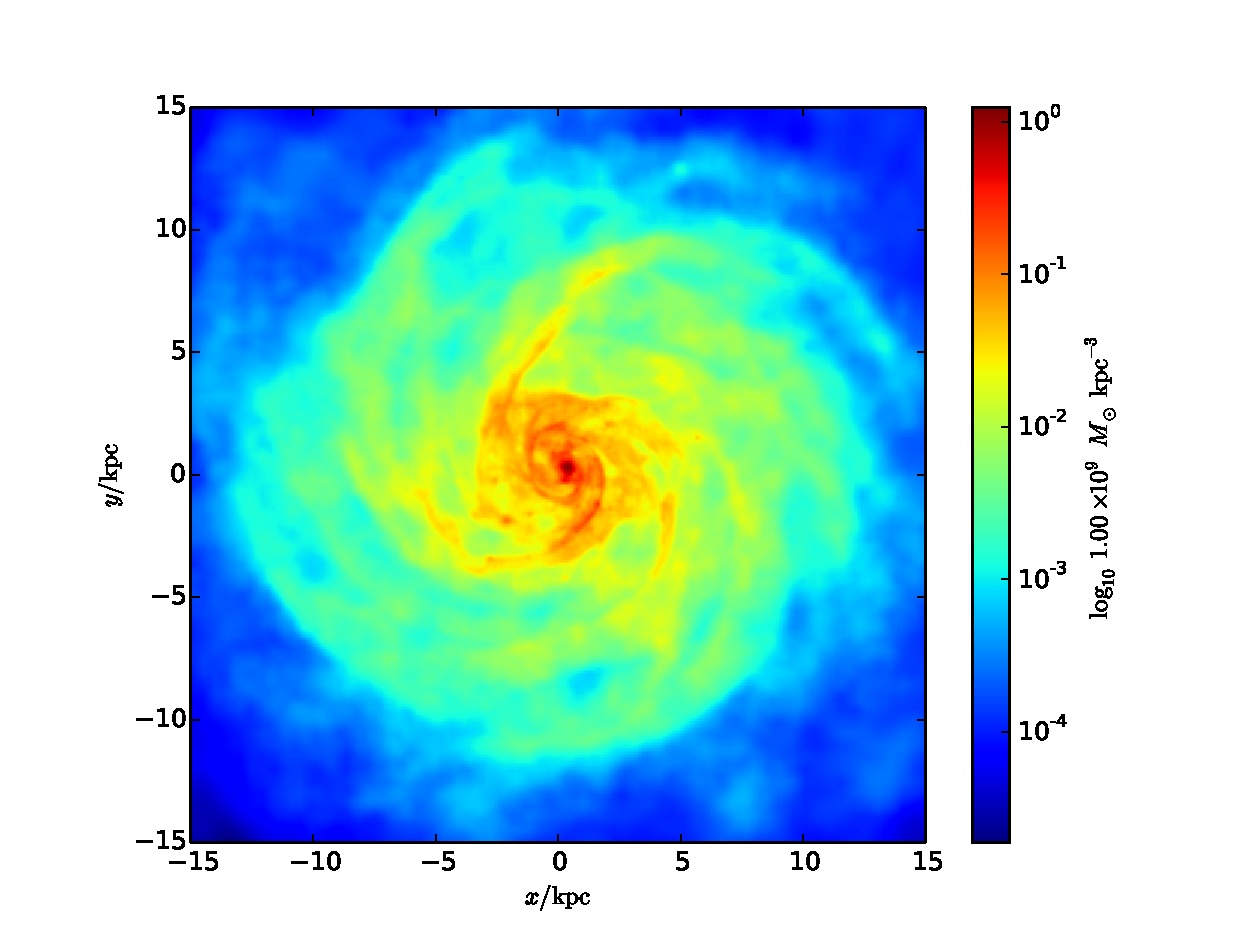
\includegraphics[width=\textwidth]{graphics/AGORAic.eps}
\caption[The AGORA IC]{A density projection of a relaxed version of the AGORA initial condition. We have run the IC for 335 Myr in order to relax it.}
\label{fig:agoraic}
\end{figure}

%notes about various runs we did

We have run the low resolution simulation with a number of different physical parameters, including our radiative transfer with FUV, a background FUV at two intensities (the standard for most codes without radiative transfer), Supernovae (SNe) feedback \citep{kellerEt14}, and a number of different opacities. Table \ref{tab:simsummary} summarizes the simulations and the names we have given them.

\begin{table}
\begin{tabular}{lllll}
Name & RT & UV Strength (units?) & Opacity (g/cm$^{-2}$) & SNe Feedback\\ \hline \hline
FUV0 & No & 0 & 0 & No\\
FUV & Yes & 0 & 300 & No\\
FUVop100 & Yes & 0 & 100 & No\\
FUVthin & Yes & 0 & 0 & No\\
FUV2e-26 & No & 2e-26 & 300 & No\\u? This is amazing and looks extremely difficult to recreate
permalink
[–]BlindStark 20 points 2 hours ago 
There is an achievement hunter video where they jump from helicopters to do
FUV2e-27 & No & 2e-27 & 300 & No\\
FB & No & ? & 300 & yes\\
FB\_FUV & Yes & 0 & 300 & yes\\
FB\_FUV2e-26 & No & 2e-26 & 300 & yes\\
FB\_FUV2-27 & No & 2e-27 & 300 & yes\\
\hline
\end{tabular}
\caption[Summary of simulations]{A summary of the simulations that were run.}
\label{tab:simsummary}
\end{table}

We attempted to match opacities given in \citet{wolfireEt03}. The left pane of figure \ref{fig:wolfiresummary} shows the midplane HI density and absorption coefficient, and the right pane is the inferred opacity from the left pane, obtained by dividing absorption by mass density.

\begin{figure}
        \centering
        \begin{subfigure}[b]{0.45\textwidth}
                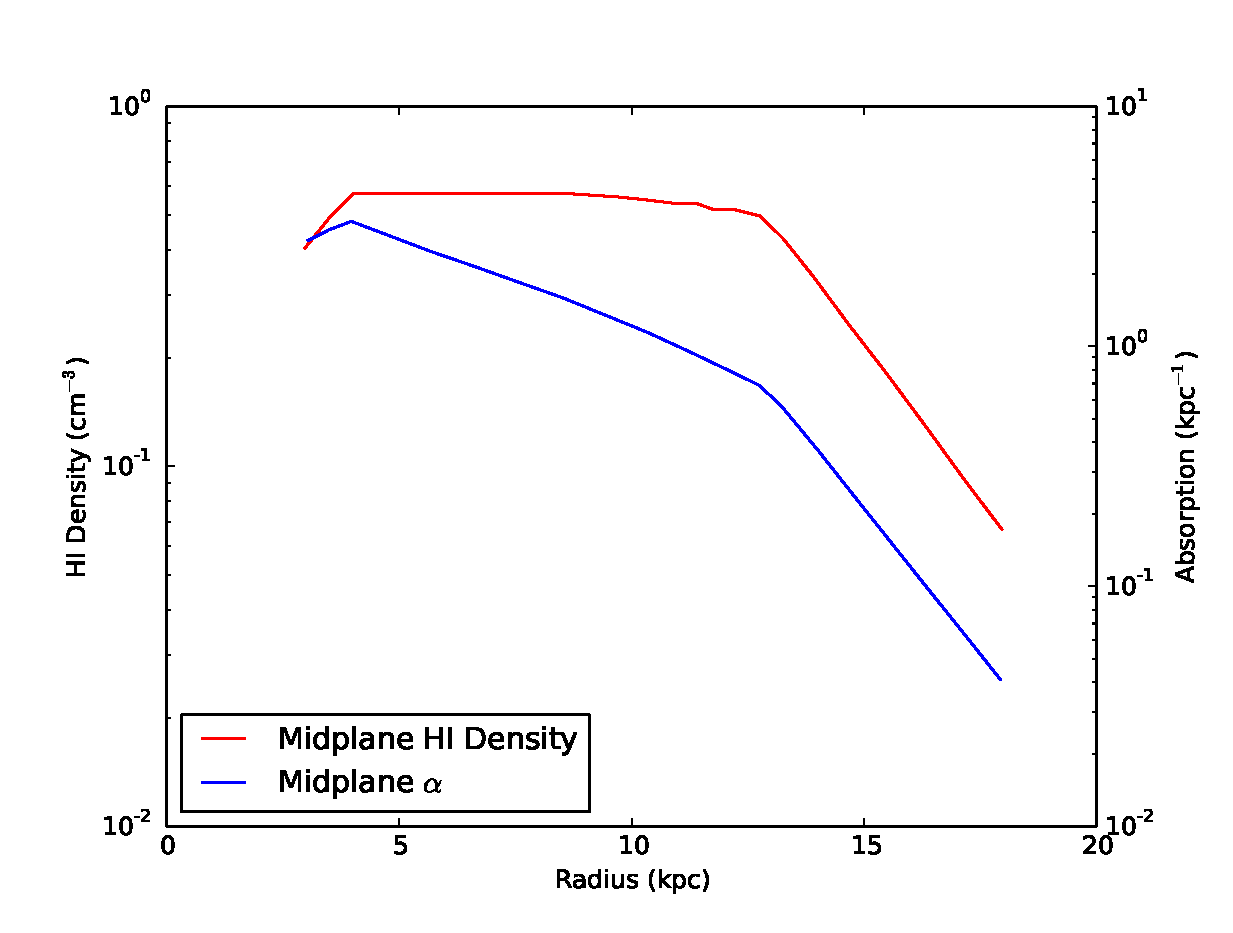
\includegraphics[width=\textwidth]{graphics/densityabsorptionvr.eps}
        \end{subfigure}
        ~ 
        \begin{subfigure}[b]{0.45\textwidth}
                \includegraphics[width=\textwidth]{graphics/opacityvr.eps}
        \end{subfigure}
        \caption[Parameters from \citet{wolfireEt03}.]{Parameters from \citet{wolfireEt03}. The left plot shows the mid plane number density and absorption coefficient. The right plot is obtained by converting number density to a mass density and dividing absorption coefficient by mass density.}
        \label{fig:wolfiresummary}
\end{figure}

Note that the profile in opacity is due solely to a scaling in metallicity of the local opacity. \citet{wolfireEt03} assume that opacity changes as

\begin{equation}
\kappa = \kappa_{\odot}\left(\frac{Z}{Z_{\odot}}\right),
\end{equation}

where $\kappa_{\odot}$ is the metallicity in the solar neighborhood, inferred to be ~400 g/cm$^{-2}$ from figure \ref{fig:wolfiresummary}.

We have also included a run at eight times higher resolution to check on convergence of results. These runs are prefixed with an ``8''.

\section{The Role of FUV on Star Formation}
\label{sec:fuvsfr}



%\begin{figure}
%        \centering
%        \begin{subfigure}[b]{0.3\textwidth}
%                \includegraphics[width=\textwidth]{graphics/surfacedensityRadFUV0_J300080.eps}
%                \caption{FUV0}
%                \label{fig:intensitythin}
%        \end{subfigure}
%        ~
%        \begin{subfigure}[b]{0.3\textwidth}
%                \includegraphics[width=\textwidth]{graphics/surfacedensityRadFUV2e-26_J300080.eps}
%                \caption{FUV2e-26}
%                \label{fig:intensity100}
%        \end{subfigure} 
%        ~ 
%        \begin{subfigure}[b]{0.3\textwidth}
%                \includegraphics[width=\textwidth]{graphics/surfacedensityRadFUVop400_J300080.eps}
%                \caption{FUVop400}
%                \label{fig:intensity100}
%        \end{subfigure}
%        \\
%        \begin{subfigure}[b]{0.3\textwidth}
%                \includegraphics[width=\textwidth]{graphics/surfacedensityRadFUV_J300080.eps}
%                \caption{FUVop300}
%                \label{fig:intensitythin}
%        \end{subfigure}
%        ~
%        \begin{subfigure}[b]{0.3\textwidth}
%                \includegraphics[width=\textwidth]{graphics/surfacedensityRadFUVop100_J300080.eps}
%                \caption{FUVop100}
%                \label{fig:intensitythin}
%        \end{subfigure}
%        ~
%        \begin{subfigure}[b]{0.3\textwidth}
%                \includegraphics[width=\textwidth]{graphics/surfacedensityRadFUVthin_J300080.eps}
%                \caption{FUVthin}
%                \label{fig:intensitythin}
%        \end{subfigure}
%        \\
%         \begin{subfigure}[b]{0.3\textwidth}
%                \includegraphics[width=\textwidth]{graphics/surfacedensityRadFB_J300080.eps}
%                \caption{FB}
%                \label{fig:intensity100}
%        \end{subfigure}
%        ~ 
%        \begin{subfigure}[b]{0.3\textwidth}
%                \includegraphics[width=\textwidth]{graphics/surfacedensityRadFB_FUV2e-26_J300080.eps}
%                \caption{FB\_FUV2e-26}
%                \label{fig:intensitythin}
%        \end{subfigure}
%        ~
%        \begin{subfigure}[b]{0.3\textwidth}
%                \includegraphics[width=\textwidth]{graphics/surfacedensityRadFB_FUV_J300080.eps}
%                \caption{FB\_FUV}
%                \label{fig:intensitythin}
%        \end{subfigure}
%        \caption[Surface density for varying runs.]{Surface density plots for the different runs.}
%        \label{fig:intensityvopacity}
%\end{figure}

%\begin{figure}
%        \centering
%        \begin{subfigure}[b]{0.45\textwidth}
%                \includegraphics[width=\textwidth]{graphics/fluximageRadFUV_J300080.eps}
%                \caption{FUVop300}
%                \label{fig:intensitythin}
%        \end{subfigure}
%        ~
%        \begin{subfigure}[b]{0.45\textwidth}
%                \includegraphics[width=\textwidth]{graphics/fluximageRadFUVthin_J300080.eps}
%                \caption{FUVthin}
%                \label{fig:intensity100}
%        \end{subfigure}        
%        \\
%        \begin{subfigure}[b]{0.45\textwidth}
%                \includegraphics[width=\textwidth]{graphics/fluximage8_RadFUV_J300080.eps}
%                \caption{8\_FUVop300}
%                \label{fig:intensitythin}
%        \end{subfigure}
%        ~
%        \begin{subfigure}[b]{0.45\textwidth}
%                \includegraphics[width=\textwidth]{graphics/fluximage8_RadFUVthin_J300080.eps}
%                \caption{8\_FUVthin}
%                \label{fig:intensitythin}
%        \end{subfigure}        
%        \\ 
%        \begin{subfigure}[b]{0.45\textwidth}
%                \includegraphics[width=\textwidth]{graphics/fluximageRadFUVop400_J300080.eps}
%                \caption{FUVop400}
%                \label{fig:intensity100}
%        \end{subfigure}
%        ~
%        \begin{subfigure}[b]{0.45\textwidth}
%                \includegraphics[width=\textwidth]{graphics/fluximageRadFB_FUV_J300080.eps}
%                \caption{FB\_FUVop300}
%                \label{fig:intensitythin}
%        \end{subfigure}    
%        \caption[Mass-weighted intensity.]{Mass-weighted intensity of the different runs.}
%        \label{fig:intensityvopacity}
%\end{figure}

We begin by looking at the star formation history of each simulation. Figure \ref{fig:sfrvtime} shows the star formation rate as a function of time for each simulation. 

%\begin{figure}
%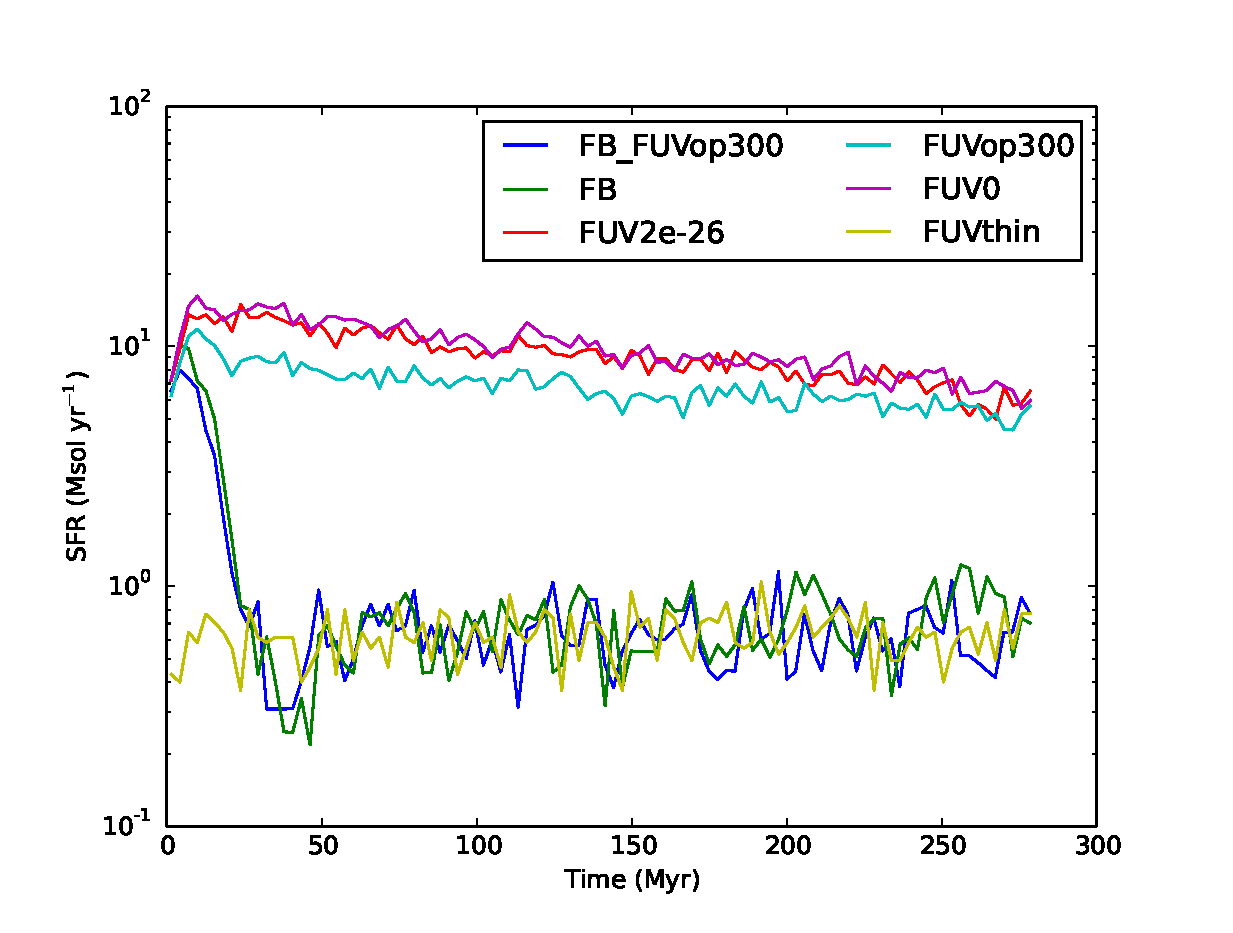
\includegraphics[width=\textwidth]{graphics/sfrvtime.eps}
%\caption[Star formation histories.]{Star formation rate vs time for each simulation. Feedback dominates the star formation regulation in this galaxy. Looking only at FUV, local feedback has a noticeable effect over a uniform background UV field.}
%\label{fig:sfrvtime}
%\end{figure}

It is clear that SNe feedback has a very strong regulation effect on star formation, as the rate in all runs with SNe feedback is about a factor of five lower than simulations without SNe feedback. In runs without SNe feedback, local FUV fields tend to reduce star formation rates by a factor of around 25\% compared to uniform backgrounds. Comparing the RadFUV2e-26 and RadFUV2e-27, there is no noticeable difference, suggesting that the FUV due to a uniform background has no ability to regulate star formation.

We must check whether the FUV field present in the galaxy is similar to observations. Figure \ref{fig:intensitywolfire} is a plot of FUV intensity vs radius in the midplane of the galaxy.

%\begin{figure}
%\includegraphics[width=\textwidth]{graphics/intensityvrRadFUV_J300080.eps}
%\caption[FUV intensity vs radius]{FUV intensity vs radius in the galaxy midplane for the RadFUV case. The dots are individual particle fluxes and the solid line is from figure 5.5 of \citet{wolfireEt03}.}
%\label{fig:intensitywolfire}
%\end{figure}

The points are intensities for individual particles and the lines is the mean intensity presented in \citet{wolfireEt03}. On average, the FUV intensity seen by a particle is far lower than the mean field presented by \citet{wolfireEt03}. We can examine the runs with varying opacity to see how this effects to local FUV intensity as well as the SFR.

%\begin{figure}
%        \centering
%        \begin{subfigure}[b]{0.45\textwidth}
%                \includegraphics[width=\textwidth]{graphics/intensityvrRadFUVop100_J300080.eps}
%                \caption{FUVop100}
%                \label{fig:intensity100}
%        \end{subfigure}
%        ~ 
%        \begin{subfigure}[b]{0.45\textwidth}
%                \includegraphics[width=\textwidth]{graphics/intensityvrRadFUVthin_J300080.eps}
%                \caption{FUVthin}
%                \label{fig:intensitythin}
%        \end{subfigure}
%        \caption[Intensity with varying opacity.]{FUV intensity vs radius in the galaxy midplane for $\kappa = 100$ g/cm$^{-2}$ and for an optically thin medium.}
%        \label{fig:intensityvopacity}
%\end{figure}

We see that opacity, not surprisingly, makes a large difference in the mean intensity seen by particles. However, what's notable is that even in the optically thin case, we are unable to attain the intensity levels reported in \citet{wolfireEt03}.

It is worth revisiting the star formation histories of the new simulations. Figure \ref{fig:sfrvtimeRT} shows the star formation histories for various runs with RT.

%\begin{figure}
%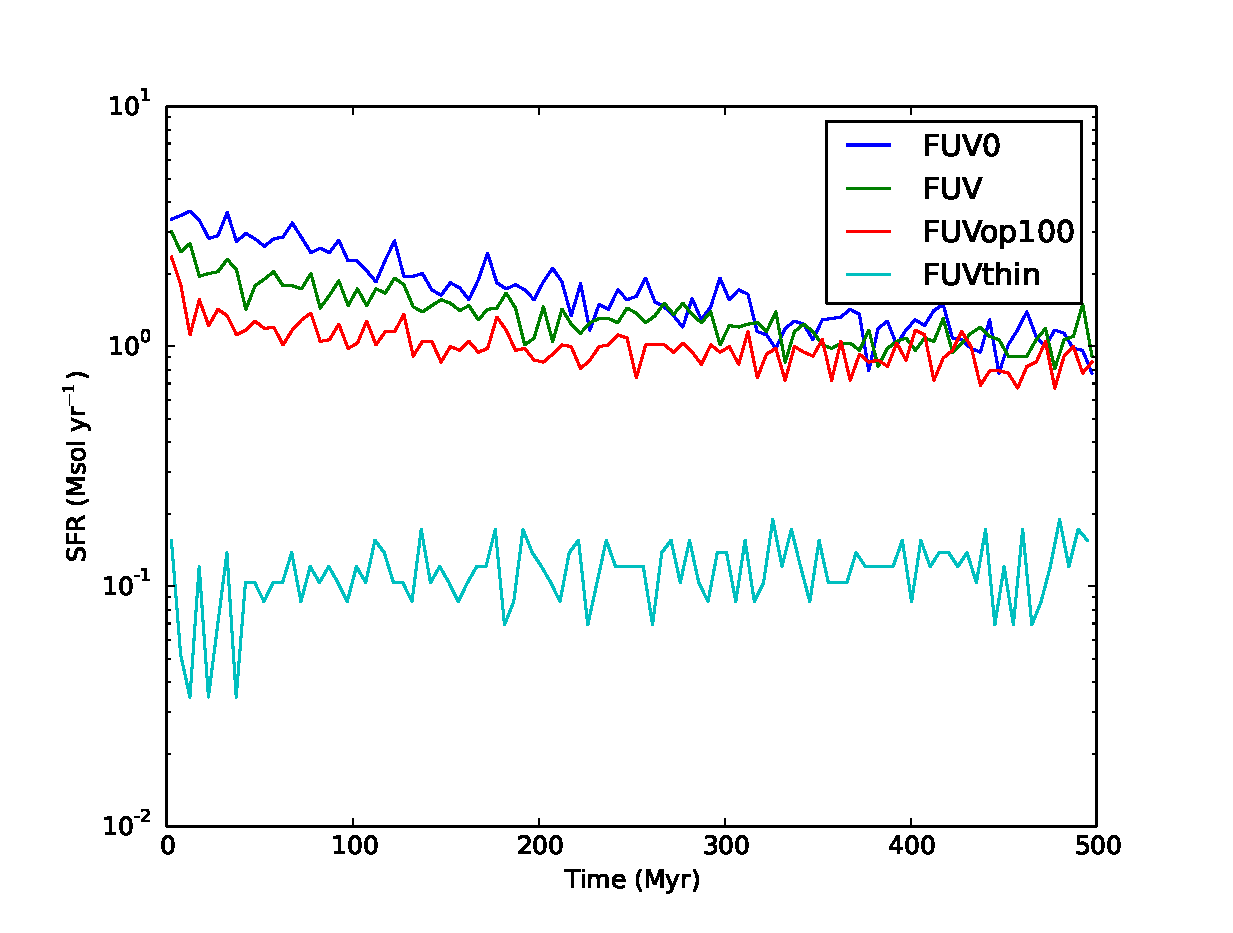
\includegraphics[width=\textwidth]{graphics/sfrvtimeRT.eps}
%\caption[Star formation histories for varying opacities.]{Star formation rate vs time with varying opacity. While the assumed opacity value of 400 g/cm,$^{-2}$ gives very minimal regulation in star formation, an optically thin approximation gives incredibly strong regulation. An opacity of 100 $g/cm^{-2}$ gives the most reasonable star formation rate, if comparing to the Milky Way.}
%\label{fig:sfrvtimeRT}
%\end{figure}

In the optically thin case, we see how important FUV can be at regulating star formation when intensities are much higher. Even lowering opacity to 100 g/cm$^{-2}$ makes a very significant difference, and gives a star formation rate in agreement with the Milky Way.

In order to understand the affect FUV has on gas, we consider phase diagrams for gas in the galaxy. Figure \ref{fig:phasediagrams} shows phase diagrams of gas in a number of the different simulations.

%\begin{figure}
%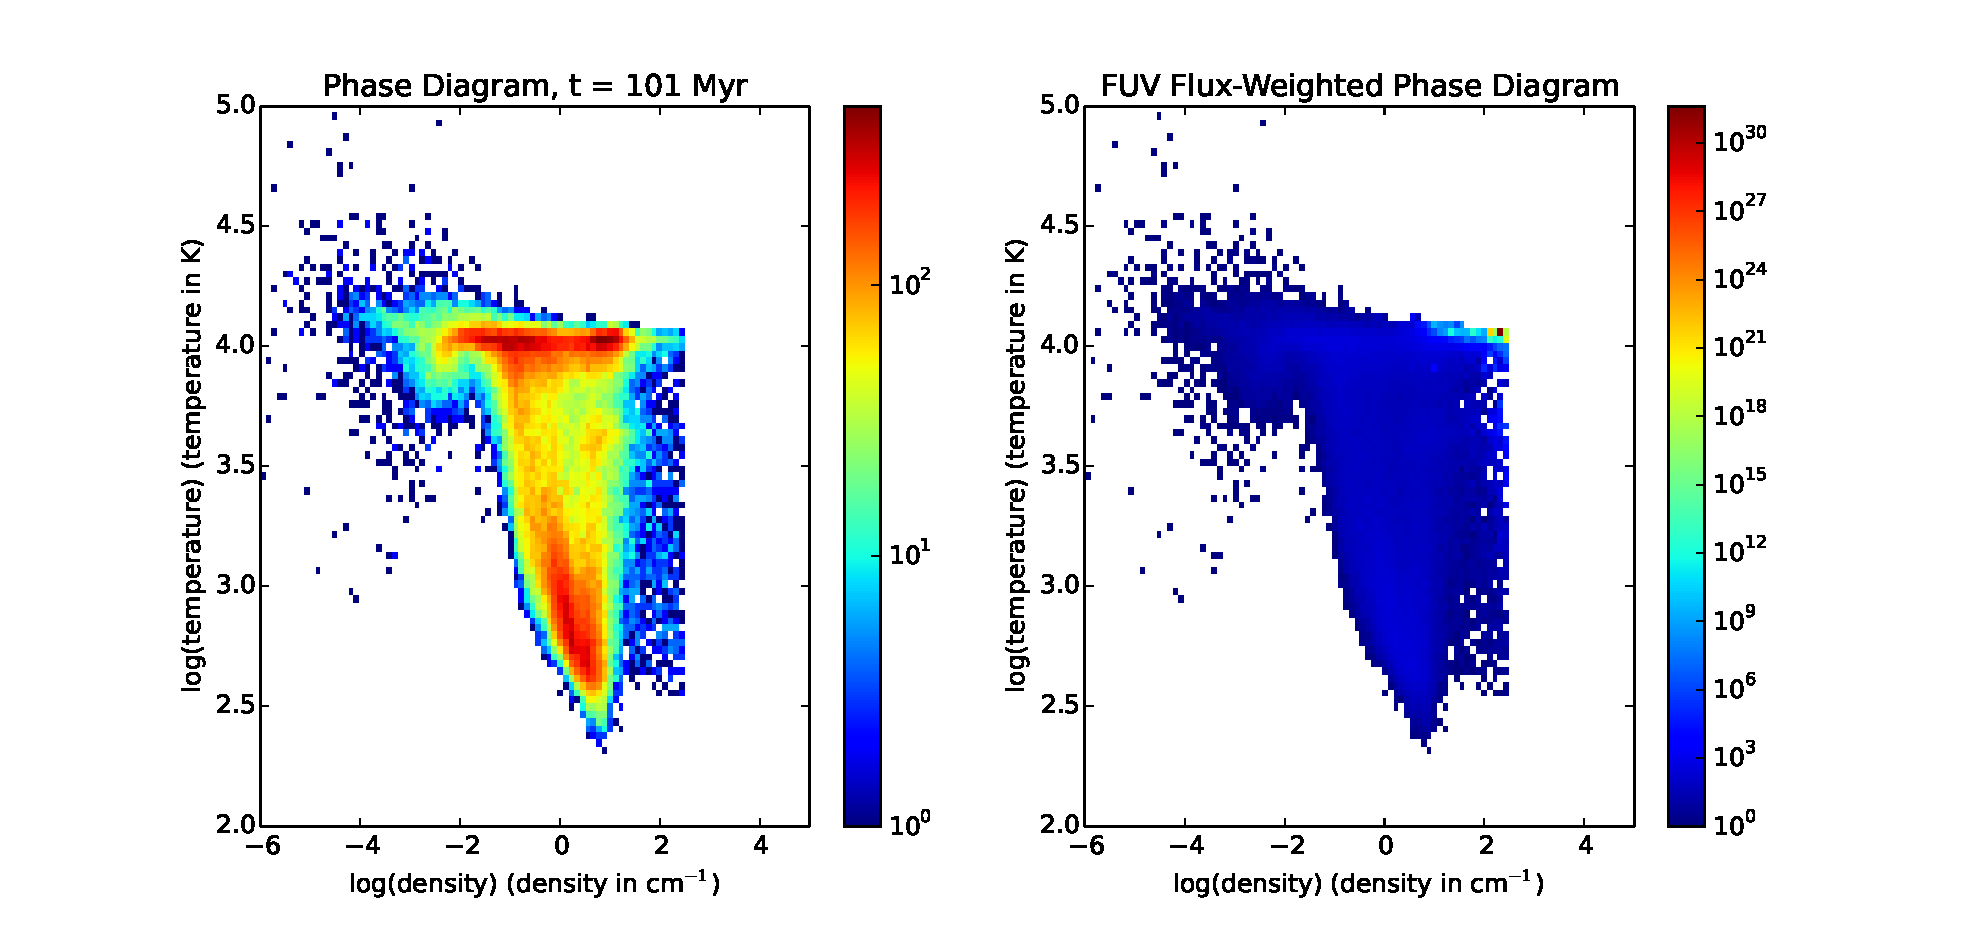
\includegraphics[width=\textwidth]{graphics/phaseRadFUV00101.eps}
%\caption[Phase diagrams with different physics]{Phase diagrams for each simulation case.}
%\label{fig:phasediagrams}
%\end{figure}

In cases with FUV simulated with radiative transfer, a portion of the gas is seen to be heated to about $10^4$ K around densities of 100 atoms cm$^{-3}$.

[Add commentary. Re-radiation important? Clumpy medium vs average opacity not the same.]
\pagestyle{fancy}
\headheight 20pt
\lhead{Ph.D. Thesis --- R. Woods }
\rhead{McMaster - Physics \& Astronomy}
\chead{}
\lfoot{}
\cfoot{\thepage}
\rfoot{}
\renewcommand{\headrulewidth}{0.1pt}
\renewcommand{\footrulewidth}{0.1pt}

\chapter{Conclusions and Future Work}
\label{chap:conclusions}
\thispagestyle{fancy}


\section{Future Projects}
\label{sec:futurework}

\subsection{Astrophysics Projects}
\label{sec:astroprojects}

Future work of this algorithm is quite broad; the flexibility allows application to a wide range of problems. An immediate follow up is to the work presented in section \ref{sec:agora}. [Author] suggests that four radiation bands, HI ionization, He ionization, LyWerner, and CI, are needed to sufficiently recreate ISM properties. Using these four bands, we would like to calculate the effect of radiation on the ISM. Including these four sources of heating and ionization will enable classification of which bands regulate star formation as a function of environment, and which bands drive particular phases of the ISM.

Currently, there is very little work in computational astrophysics that models the UV fields in and around galaxies. While many models have been created from the observational side [references], due to large computational cost, simulations have left this area largely unexplored or explored only at high redshift [references].

The next project for the radiative transfer code will be to include UV in the McMaster Unbiased Galaxy Simulations 2 (MUGS2) simulations. The MUGS2 project is a set of cosmological simulations of galaxies spanning a large range of parameter space. There are currently [16] galaxies in the set spanning a mass range of $5\e{11} M_{\odot}$ to $2\e{12} M_{\odot}$. Including explicit radiative transfer in these cosmological simulations all the way down to redshift zero would be an unprecedented accomplishment in computational galaxy formation. The group of simulations would enable comparison of the effectiveness of radiative transfer in transforming and regulating galaxy formation across a wide mass range at different epochs in time.

Having a wide range of simulated galaxies all with RT will also enable a plethora of other analysis. Currently, escape fractions of radiation from galaxies are typically assumed to be certain values (e.g. \citet{kannanEt14}). With the MUGS2 simulations including RT, escape fractions could be explicitly calculated.

\textsc{Gasoline} has a chemical network for molecular Hydrogen (H2) creation and destruction \citep{christensenEt12}, but requires an accurate Lyman-Werner field in order to be used. The new RT can provide this, and enables studies on H2 formation and destruction in galaxies, as well as studies of H2 shielding, self and dust, in molecular clouds. This has the additional advantage of easily being linked to observations.

We note that a potential application is to study cosmic re-ionization. However, this application may not be as ideal. Besides having already received a fair bit of attention from simulators, our code does not explicitly conserve photons and so does not guarantee correct ionization front propagation speeds, which are quite important for studies of cosmic re-ionization.

Finally, an exciting potential application is to look at re-radiation of photons from gas. This could include the effects of gas re-radiating ionizing photons when electrons recombine back to the ground state. This effectively increases the penetration depth of ionizing photons and can have an important effect on the gas in the ISM at particular densities [cite rahmati]. As well, processing of stellar emission down to IR wavelengths could be a very interesting study. However, both of these applications rely on a successful implementation of gas radiation in \textsc{Gasoline}. While in principle the implemented RT can handle any radiation, allowing gas to radiate requires care in that it must be self-consistently tied to the cooling that gas experiences. At first glance, separating cooling and cooling radiation induces a cooling instability and so requires further investigation to be done properly (see section \ref{sec:codeadditions}).

\subsection{Code Additions}
\label{sec:codeadditions}

The algorithm we have presented is very flexible, efficient, and powerful. However, there is a lot of room for improvement in the algorithm and optimizations that can be made.

For example, if it is know a priori that all sources lie outside of the absorbing material, the algorithm can be simplified to run in order $N\log{N}$ time by implementing the algorithm presented in TreeCOL \citep{clarkEt12}. In this scenario, each receiving leaf partitions the rest of the tree into equal areas on the sky (TreeCOL uses the HEALPIX algorithm \citep{gorskiEt05}, but it is not required) during the tree walk. Since an effective size of each cell the leaf interacts with can be calculated, each cell can add its absorption contributions to the proper area on the leaf's sky map.

It is also possible to make optimizations in the tree build process. Currently, the tree is rebuilt for every substep the simulation takes, regardless of how large the time step is. It's possible to simply ``fix'' the tree rather than rebuilding it in cases where particles have not moved by much [cite codes that do this]. Along the same lines, it's also possible to avoid recalculating radiation if the time step is very small. If particles have not moved by much and radiation sources have not been significantly changed, than there is no reason to recalculate the radiation field. This would require flagging of ``unimportant'' regions or including a radiation-set time step in the code. If the code time step was smaller than the radiation time step, then the radiation calculation could be skipped.

Currently, the algorithm supports an arbitrary number of wave bands. However, work is still needed to couple the photons in these bands to cooling and heating processes in the code. Adding this functionality will greatly open up the number of projects the algorithm can be used for.

It would also be very interesting to create the ability to use gas particles as sources. This enables the code to treat re-radiation by gas, dust emission, and potentially even scattering if a gas particle's emission in one band was based on its incident intensity in another band. Due to the excellent scaling with the number of sources that the algorithm provides, this should not be computationally prohibitive. The consideration to make here is how self consistent the cooling is with radiation. For example, if a gas particle emits a certain luminosity in certain bands, but the cooling code integrates out a different cooling rate, energy conservation can be violated, and cooling instabilities in the gas particle can be created [more details here]. This code addition will require special attention to get right.

Other minor features can be added without too much difficulty. For example, radiation is currently not allowed to be periodic. However, there is no reason a tree cell cannot be copied in a similar way to gravitational periodicity (where an offset is simply added to each cell in the tree to represent a periodic copy). As well, it is possible to add dynamical effects due to radiation such as radiation pressure. This simply requires code to be added into the acceleration calculations to use the radiation field information.

[closing statement?]

\section{Conclusions}
\label{sec:conclusion}

Deep thoughts here.

%\end{singlespace}
\end{doublespace}


%%%%%%%%%%%%%%%%%%%%%%%%%%%%%%%%%%%%%%%%%%%%%%%%%%%%%%%%%%%%%%%
%Appendices
%%%%%%%%%%%%%%%%%%%%%%%%%%%%%%%%%%%%%%%%%%%%%%%%%%%%%%%%%%%%%%%
\appendix
\pagestyle{fancy}
\headheight 20pt
\lhead{PhD Thesis --- R. Woods }
\rhead{McMaster Physics and Astronomy}
\chead{}
\lfoot{}
\cfoot{\thepage}
\rfoot{}
\renewcommand{\headrulewidth}{0.1pt}
\renewcommand{\footrulewidth}{0.1pt}

\chapter{Appendix A} \label{Appendix-A} 
\thispagestyle{fancy} 






%%%%%%%%%%%%%%%%%%%%%%%%%%%%%%%%%%%%%%%%%%%%%%%%%%%%%%%%%%%%%%%
% ESM students need to include a Nontechnical Abstract as the %
% last appendix.                                              %
%%%%%%%%%%%%%%%%%%%%%%%%%%%%%%%%%%%%%%%%%%%%%%%%%%%%%%%%%%%%%%%
% This \include command should point to the file containing
% that abstract.
%\include{nontechnical-abstract}
%%%%%%%%%%%%%%%%%%%%%%%%%%%%%%%%%%%%%%%%%%%
% End of the \allowdisplaybreak command %
%%%%%%%%%%%%%%%%%%%%%%%%%%%%%%%%%%%%%%%%%%%
}


%%%%%%%%%%%%%%%%
% BIBLIOGRAPHY %
%%%%%%%%%%%%%%%% 
% You can use BibTeX or other bibliography facility for your
% bibliography. LaTeX's standard stuff is shown below. If you
% bibtex, then this section should look something like:
\begin{singlespace}
  
  \pagestyle{fancy}
  \headheight 20pt
  \lhead{Ph.D.~Thesis - R.~Woods}
  \rhead{McMaster - Physics and Astronomy}
  \chead{}
  \lfoot{}
  \cfoot{\thepage}
  \rfoot{}
  \renewcommand{\headrulewidth}{0.1pt}
  \renewcommand{\footrulewidth}{0.1pt}
  \thispagestyle{fancy}
  
  \bibliography{thesis}
% \bibliographystyle{ieeetr}
%  \bibliographystyle{apj}
%  \bibliographystyle{plain}
  \bibliographystyle{plainnat}
  \nocite{*}
  
  \addcontentsline{toc}{chapter}{Bibliography}
  
  \thispagestyle{fancy}
  
\end{singlespace}


\end{document}
